\documentclass[handout]{beamer}
\usepackage[utf8]{inputenc}
\usepackage{graphicx}
\graphicspath{{images/}}
\usepackage[misc]{ifsym}
\usepackage[backend=biber,style=numeric, citestyle=ieee]{biblatex}
\addbibresource{IEEEexample.bib}
\AtBeginBibliography{\small}
\usepackage{appendixnumberbeamer}
\pdfstringdefDisableCommands{%
\def\translate#1{#1}%
}
% If you don't need the control symbol, uncomment it
%\beamertemplatenavigationsymbolsempty
%\usepackage{MnSymbol}
%\usepackage{tikz}
%\usetikzlibrary{arrows,shapes}
%\usepackage{stmaryrd}
%%\usepackage[utf8]{vietnam}
%
\usetheme{Berlin}
\useinnertheme{circles}
%
\AtBeginSection[]
{
  \begin{frame}
    \frametitle{Table of Contents}
    \tableofcontents[currentsection]
  \end{frame}
}
%
%Information to be included in the title page:
\title[Congressional Tweet Analysis]{Congressional Tweet Analysis}
%\subtitle{}
\author[Steve Schluchter]{Steve\inst{1}}
\institute[SQL Anonymous :)]{  
\inst{1}%
  SQL Anonymous
}
%\date[Short conference, Year]{Full Conference, Month Year }
%\logo{\includegraphics[height=.6cm]{IU}}
%
% Page number
\expandafter\def\expandafter\insertshorttitle\expandafter{%
  \insertshorttitle\hfill%
  \insertframenumber\,/\,\inserttotalframenumber}
%
\begin{document}
% Title page
\frame{\titlepage}
% ToC page
\begin{frame}{Table of Contents}
	\tableofcontents
\end{frame}
% EX: Highlighted frame with link to appendix
%\begin{frame}[label=frame]{Sample frame title}
%
%In this slide, some important text will be
%\alert{highlighted} because it's important.
%Please, don't abuse it.
%
%\begin{block}{Remark}
%Sample text
%\end{block}
%
%\begin{alertblock}{Important theorem}
%Sample text in red box
%\end{alertblock}
%
%\begin{examples}
%Sample text in green box. The title of the block is ``Examples".
%\end{examples}
%\hyperlink{appendix}{\beamerbutton{More on Appendix}}	
%\end{frame}
% EX: Two column frame
%\begin{frame}{Two-column slide}
%\begin{columns}
%\column{0.5\textwidth}
%This is a text in first column.
%$$E=mc^2$$
%\begin{itemize}
%\item First item
%\item Second item
%\end{itemize}
%
%\column{0.5\textwidth}
%This text will be in the second column
%and on a second thoughts, this is a nice looking
%layout in some cases.
%\end{columns}
%\end{frame}
% EX: Sample frame with effects
%\begin{frame}{Title frame 1}
%\begin{block}{Block blue}
%\begin{itemize}
% \item<1-> Text visible on slide 1
% \item<2-> Text visible on slide 2
% \item<3> Text visible on slide 3
% \item<4-> Text visible on slide 4
%\end{itemize}
%\end{block}  
%\end{frame}
% EX: Sample frame with Math eq.
%\begin{frame}{Title Frame 2}
%In this slide \pause
%the text will be partially visible \pause
%And finally everything will be there
%\[\ support(X \to Y) = p(X \cup Y) = \frac{{n(X \cup Y)}}{N}\]
%\end{frame}

\section{30000 ft overview}  
% Thank you frame
\begin{frame}\frametitle{some high level statistics}
	\flushleft
    \visible<1->{There are $1243370$ total tweets.\\ \smallskip}
    \visible<1->{There are $545$ different screen names among the data.\\ \smallskip}
    \visible<1->{The earliest tweet is indexed at 2008-08-04 and the latest tweet is indexed at 2017-06-06.\\ \smallskip}
\end{frame}

\section{Two AB Tests}
\begin{frame}\frametitle{What makes a tweet more retweetable?}
\flushleft

\visible<1->{$\bullet$ We ran multiple AB tests on the impact of the sentiment score on a tweet getting retweeted.\\ \smallskip}
\visible<2->{$\bullet$ We considered the impact of scores higher than $0.1$, $0.2$, $0.3$, $\ldots$, $0.9$, and the answer was decidedly no.  In each case, we failed to reject the null hypothesis that the sentiment score had a slightly negative impact on a tweet being retweeted.\\ \smallskip}
\visible<3->{$\bullet$ We also considered the presence of a \#hashtag in the tweet as an indicator of a tweet getting retweeted.  The answer was overwhelmingly yes.}
\end{frame}

\begin{frame}\frametitle{Does emotionality make a tweet more retweetable?}
\flushleft
\visible<1->{Not for sentiment score of greater than $0.1$.}
\visible<1->{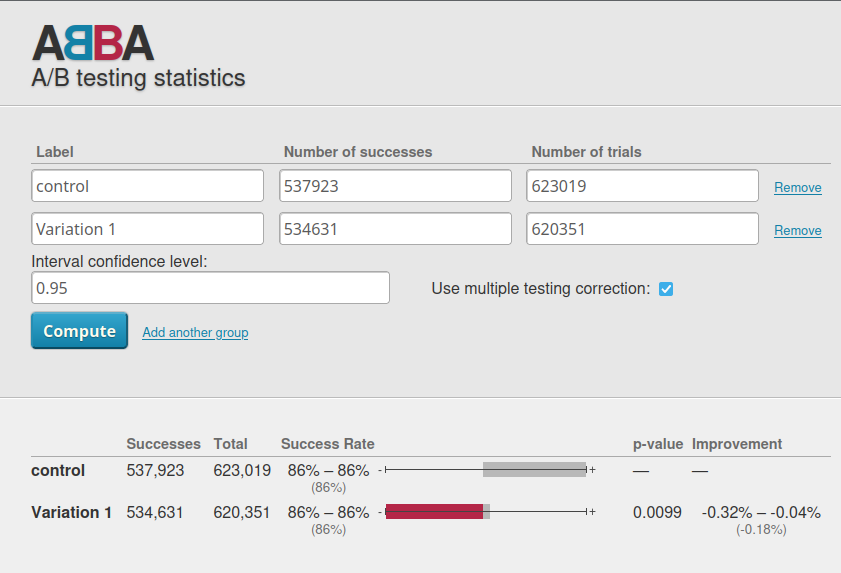
\includegraphics[scale=0.4]{Screenshot_test_0.1.png} \smallskip}

\end{frame}

\begin{frame}\frametitle{Does emotionality make a tweet more retweetable?}
\flushleft

\visible<1->{Not for sentiment score of greater than $0.2$.}

\visible<1->{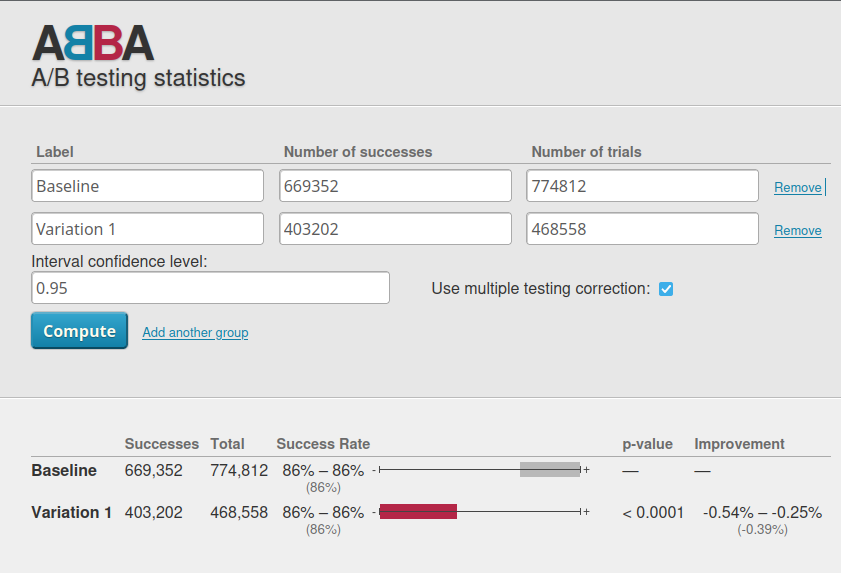
\includegraphics[scale=0.4]{Screenshot_test_0.2.png} \smallskip}

\end{frame}

\begin{frame}\frametitle{Does emotionality make a tweet more retweetable?}
\flushleft

\visible<1->{Not for sentiment score of greater than $0.3$.}

\visible<1->{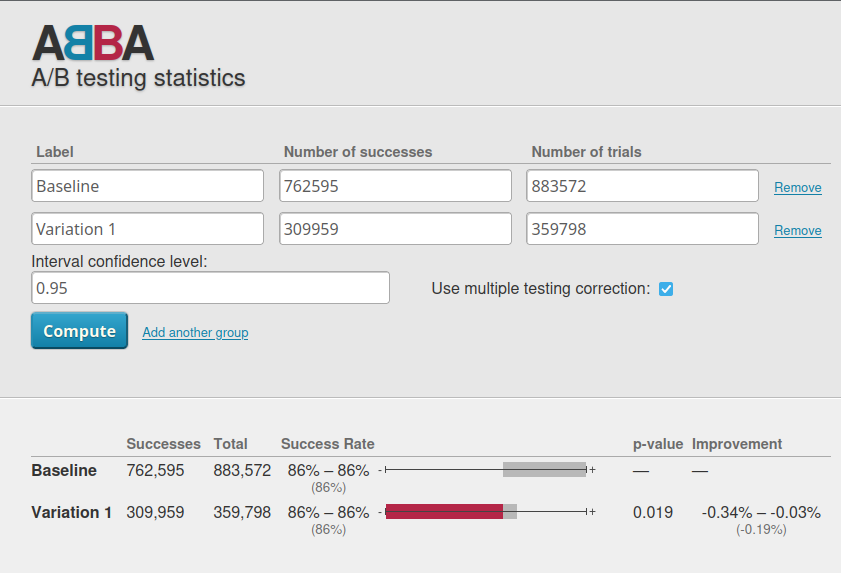
\includegraphics[scale=0.4]{Screenshot_test_0.3.png} \smallskip}

\end{frame}

\begin{frame}\frametitle{Does emotionality make a tweet more retweetable?}
\flushleft

\visible<1->{Not for sentiment score of greater than $0.4$.}

\visible<1->{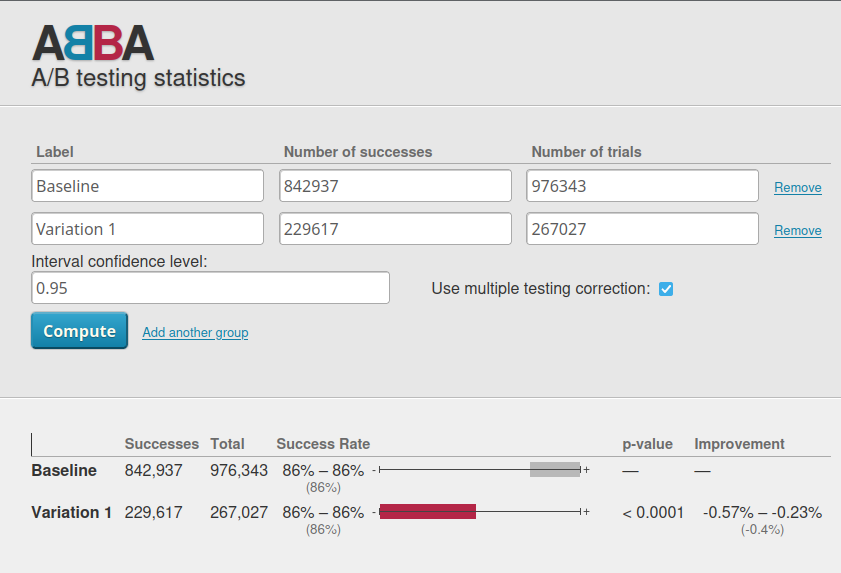
\includegraphics[scale=0.4]{Screenshot_test_0.4.png} \smallskip}

\end{frame}

\begin{frame}\frametitle{Does emotionality make a tweet more retweetable?}
\flushleft

\visible<1->{Not for sentiment score of greater than $0.5$.}

\visible<1->{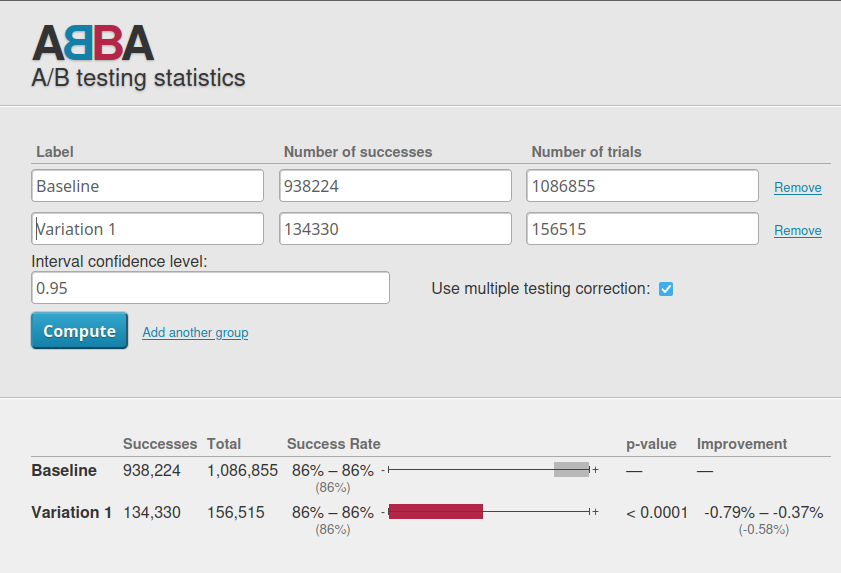
\includegraphics[scale=0.4]{Screenshot_test_0.5.png} \smallskip}

\end{frame}

\begin{frame}\frametitle{Does emotionality make a tweet more retweetable?}
\flushleft

\visible<1->{Not for sentiment score of greater than $0.6$.}


\visible<1->{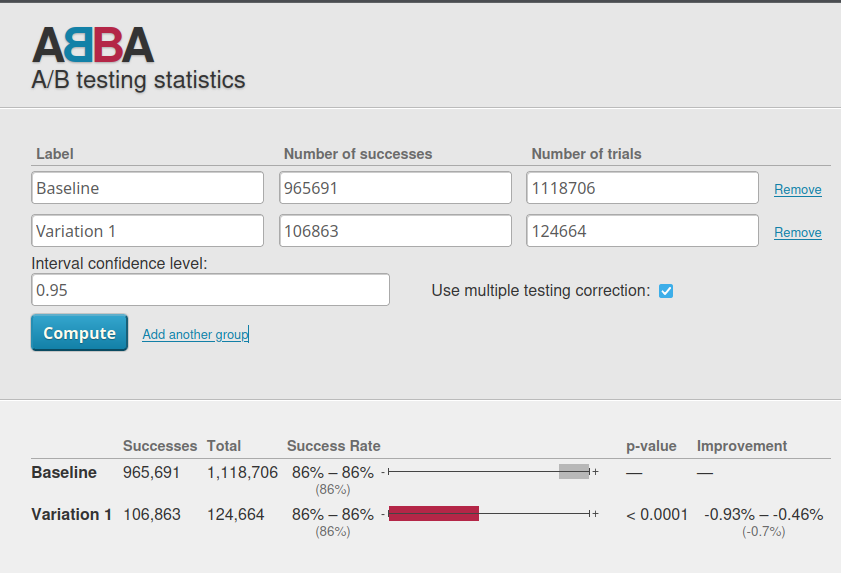
\includegraphics[scale=0.4]{Screenshot_test_0.6.png} \smallskip}

\end{frame}

\begin{frame}\frametitle{Does emotionality make a tweet more retweetable?}
\flushleft

\visible<1->{Not for sentiment score of greater than $0.7$.}

\visible<1->{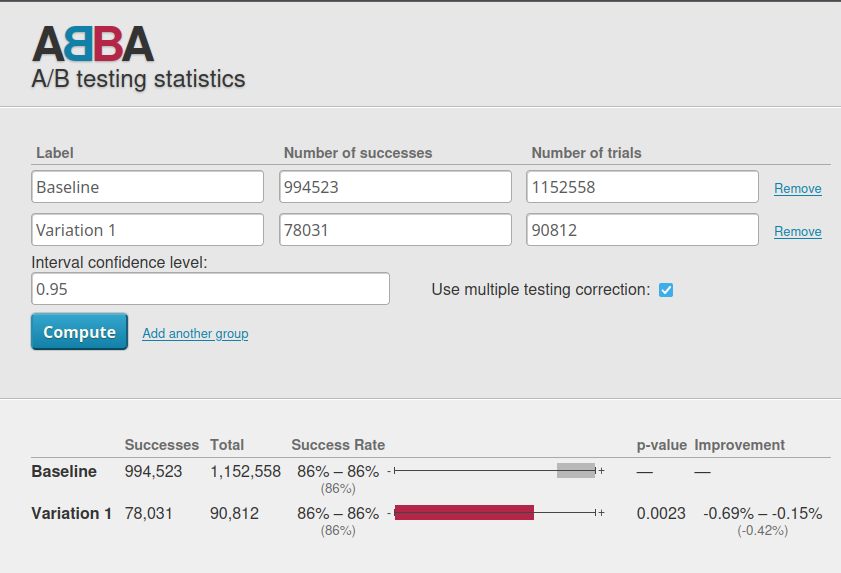
\includegraphics[scale=0.4]{Screenshot_test_0.7.png} \smallskip}

\end{frame}

\begin{frame}\frametitle{Does emotionality make a tweet more retweetable?}
\flushleft

\visible<1->{Not for sentiment score of greater than $0.8$.}

\visible<1->{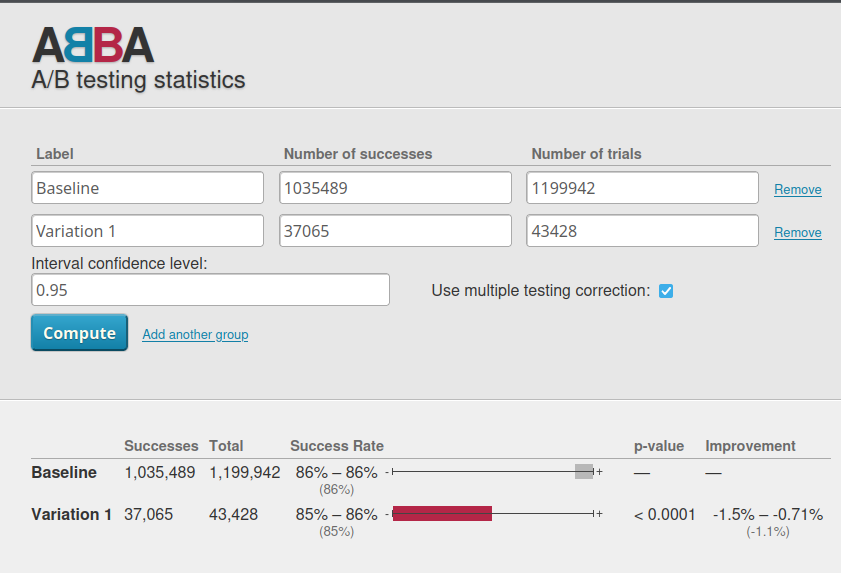
\includegraphics[scale=0.4]{Screenshot_test_0.8.png} \smallskip}

\end{frame}

\begin{frame}\frametitle{Does emotionality make a tweet more retweetable?}
\flushleft

\visible<1->{Not for sentiment score of greater than $0.9$.}

\visible<1->{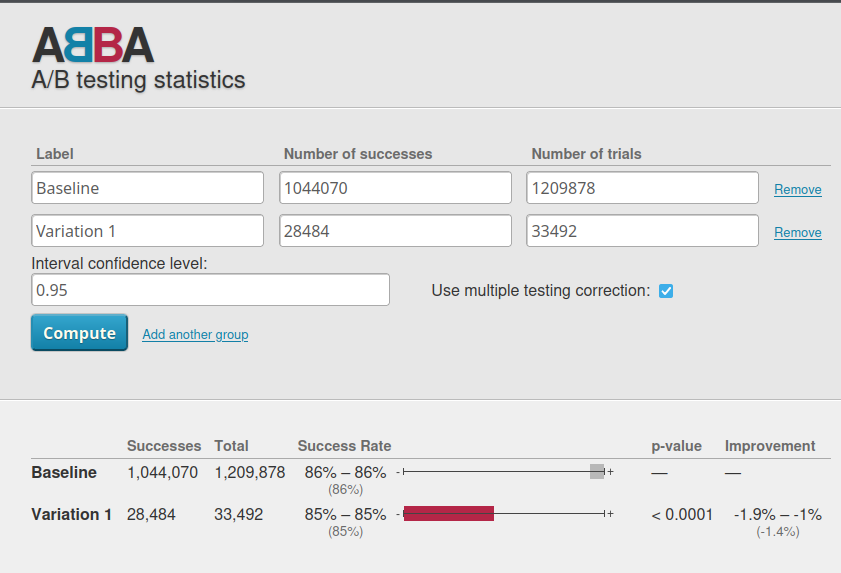
\includegraphics[scale=0.4]{Screenshot_test_0.9.png} \smallskip}

\end{frame}

\begin{frame}\frametitle{Do \#hashtags make a tweet more retweetable?}
\flushleft
\visible<1->{Yes, they do!}
\visible<1->{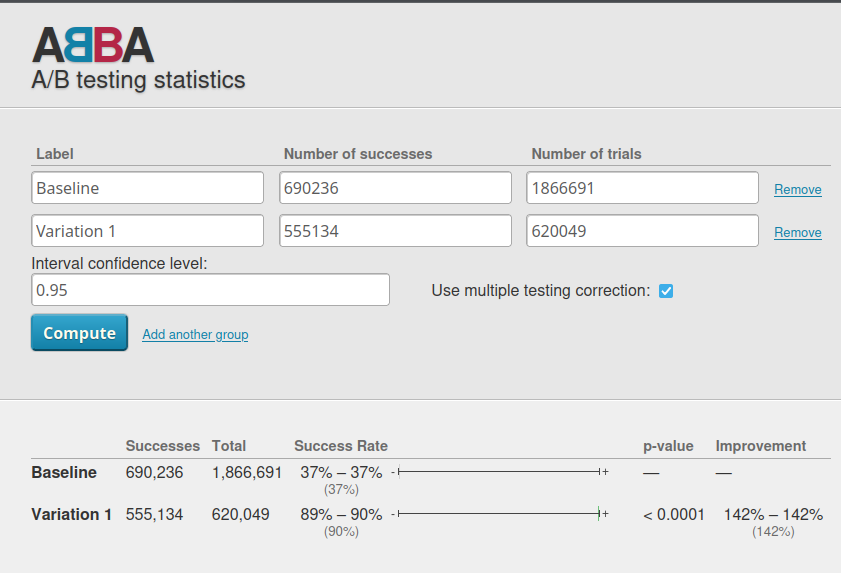
\includegraphics[scale=0.4]{Screenshot_hashtags.png} \smallskip}

\end{frame}


\section{The most popular user on Twitter?}
\begin{frame}\frametitle{It depends on how you count it}
\flushleft

\visible<1->{First, a heatmap matrix of the Pearson correlation coefficients of some user data.\\}
\visible<1->{This illuminates which popularity measures are related to which.\\}
\centering
\visible<1->{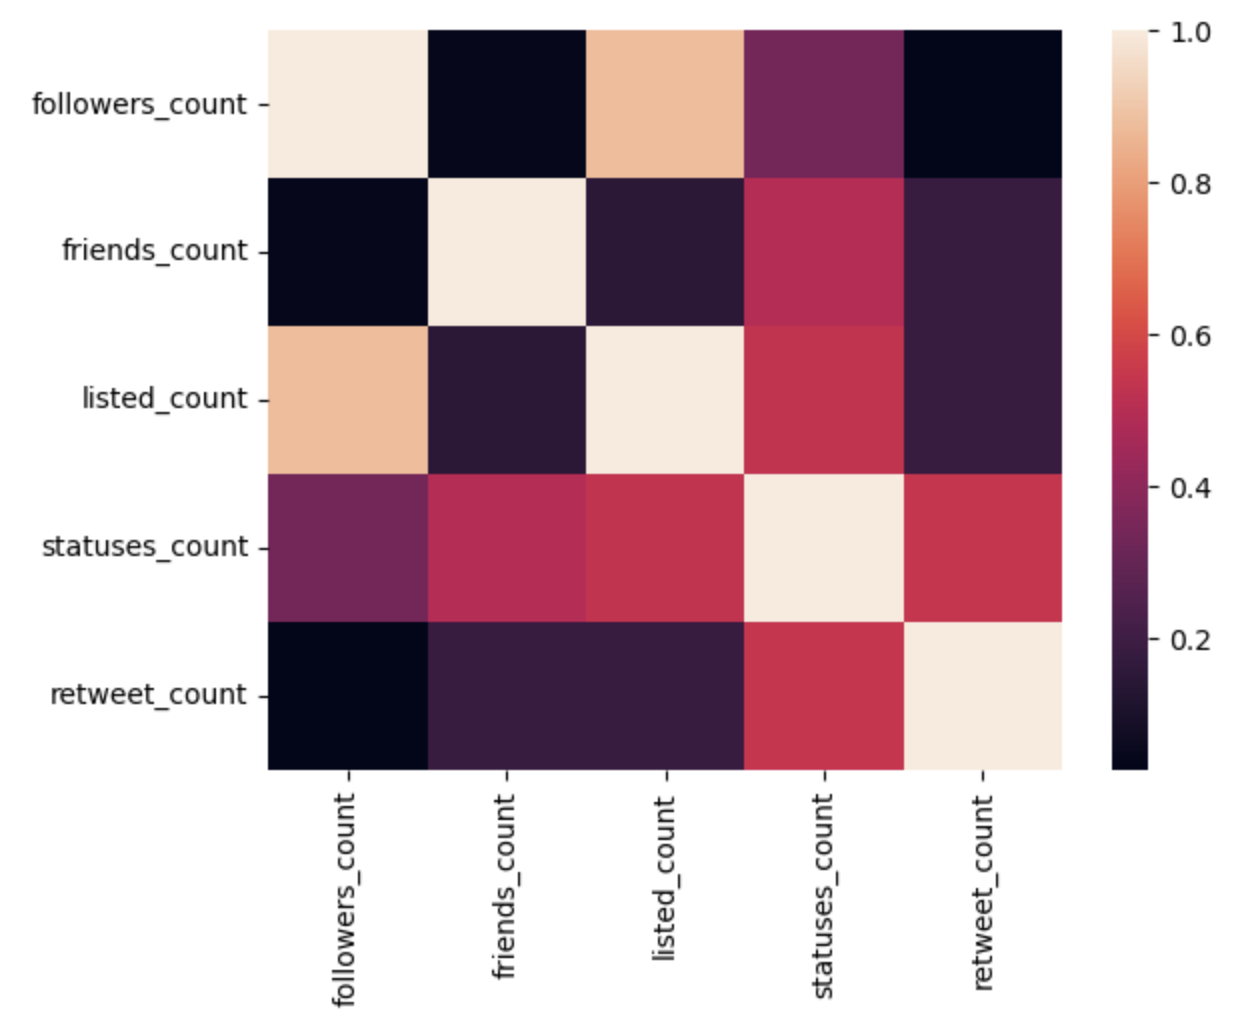
\includegraphics[scale=0.25]{heatmap.png}}

\end{frame}

\begin{frame}\frametitle{It depends on how you count it}
\flushleft
\visible<1->{We focus on retweets.  We could have counted friends, etc..\\}
\visible<1->{Here are the top $20$ accounts, sorted by number of retweets, in descending order.\\}
\visible<1->{\centering 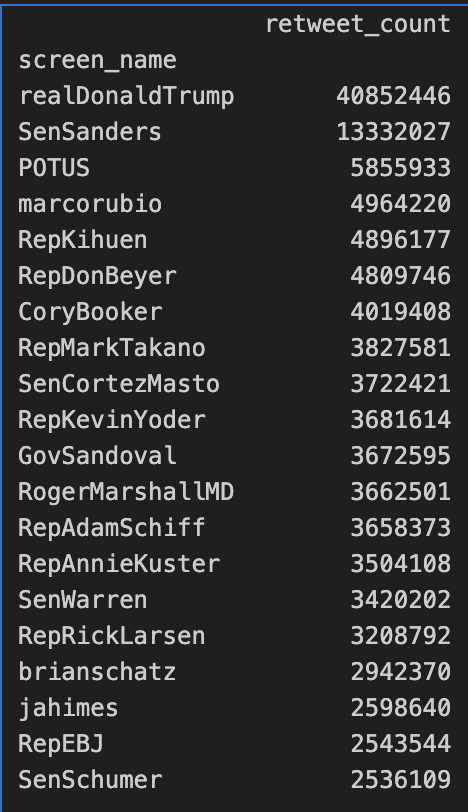
\includegraphics[scale=0.3]{top_20_accounts.png}}
\end{frame}

\begin{frame}\frametitle{It depends on how you count it}
\flushleft
\visible<1->{We build a directed graph where a directed edge from one node to another means that a Twitter user tweeted at another twitter user.  Here are the top $20$ nodes according to the number of edges directed toward those nodes.\\}
\visible<1->{\centering 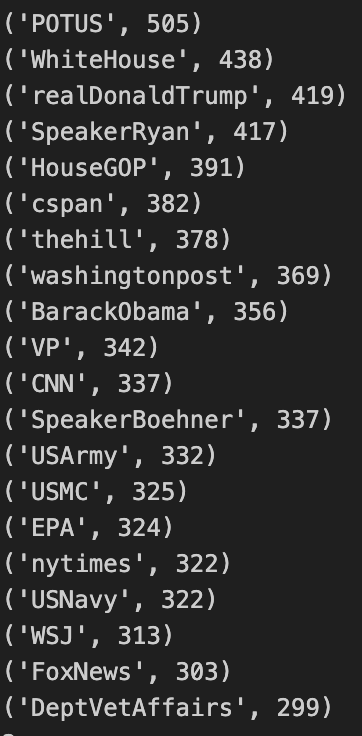
\includegraphics[scale=0.3]{Top_20_nodes.png}}

\end{frame}



\begin{frame}\frametitle{Thank you!}
\flushleft
\visible<1->{\centering $\bullet$ In any timezone! $\bullet$}
\end{frame}

% Appendix frame(s)
%\appendix
% EX: Appendix frame with link to frame
%\begin{frame}[label=appendix]{Sample frame title}
%
%In this slide, some important text will be
%\alert{highlighted} because it's important.
%Please, don't abuse it.
%
%\begin{block}{Remark}
%Sample text
%\end{block}
%
%\begin{alertblock}{Important theorem}
%Sample text in red box
%\end{alertblock}
%
%\begin{examples}
%Sample text in green box. The title of the block is ``Examples".
%\end{examples}
%\hyperlink{frame}{\beamerbutton{Back to Frame}}	
%\end{frame}
% Reference frame

\end{document}
